% !TEX program = lualatex
\documentclass[11pt, letterpaper]{article}

\usepackage{amsmath}
\usepackage{modern}
\usepackage{graphicx}
\usepackage{booktabs}
\usepackage{seqsplit}
\usepackage{todonotes}

% modern.sty sets 1.25in side margins; widen the margin-note box so notes
% are readable (default marginparwidth is too narrow and todonotes warns).
\setlength{\marginparwidth}{2.4cm}

% Repository paths inside provenance notes. \seqsplit lets a long path break
% anywhere, so it fits the narrow margin box instead of overflowing it. Never
% put a space inside \pth: \seqsplit discards it.
%
% Must be robust: todonotes writes every note's text to the .tdo file for
% \listoftodos, and \seqsplit expands to garbage if it is written unprotected.
\DeclareRobustCommand{\pth}[1]{\texttt{\seqsplit{#1}}}

% Provenance-note commands.
\newcommand{\srcnote}[2][]{\todo[color=blue!15,size=\scriptsize,#1]{#2}}    % SRC, DATA
\newcommand{\calcnote}[2][]{\todo[color=green!15,size=\scriptsize,#1]{#2}}  % CALC, FIG
\newcommand{\kbnote}[2][]{\todo[color=orange!20,size=\scriptsize,#1]{#2}}   % KB, ASSUME
\newcommand{\checknote}[2][]{\todo[color=red!20,size=\scriptsize,#1]{#2}}   % CHECK

\addbibresource{references.bib}

\title{The Monthly Average 7:00 a.m.\ Dew Point at Bryan, Texas:\\
Two Years of Observation and a Twelve-Month Probabilistic Forecast}
\author{Henry Bryant}
\date{31 August 2026}

\begin{document}

\maketitle
\thispagestyle{empty}

\begin{abstract}
\noindent
This report documents the monthly average 7:00 a.m.\ dew point at Bryan, Texas,
over the two years ending August 2026, and presents a probabilistic forecast of
that quantity for the twelve months from September 2026 through August 2027.
The series is constructed from routine hourly observations at Coulter Field
(KCFD), the automated weather station inside the Bryan city limits. The forecast
comes from a seasonal harmonic model with a multiplicative seasonal variance
term and a first-order autoregressive anomaly, simulated forward with
bootstrapped innovations. The central result about the forecast is negative and
worth stating plainly: at a monthly horizon this variable carries almost no
exploitable persistence, so the forecast is close to a seasonal climatology with
an honest, strongly season-dependent measure of dispersion. Its width is the
substantive content. The 80~percent interval spans 3.9\,\textdegree{}F in July
2027 and 15.2\,\textdegree{}F in January 2027.\footnote{%
This report was produced in response to the following prompt: ``Create a report
in this directory. Call this `dew\_point'. Use the `soothfast' writing
instructions in the \url{https://github.com/h-bryant/latex-tools} repo. The
report should present a figure showing the evolution of the average monthly 7:00
AM dew point in Bryan, Texas, over the last two years, and a fan graph depicting
a probabilistic forecast for that monthly value for the coming 12 months.
Include this prompt in the a footnote.'' The prompt is reproduced verbatim,
including its typographical errors.}
\end{abstract}

\calcnote[inline]{CALC: abstract figures restate results derived below; see the
notes in Sections 3--6. Interval widths from
\pth{analysis/dewpoint\_forecast/output/model\_summary.txt}, block
\texttt{[forecast]}.}

\section{Purpose and scope}

The quantity of interest is the dew point temperature recorded at 7:00 a.m.\
local time at Bryan, Texas, averaged within each calendar month. The dew point
is the temperature to which air must be cooled, at constant pressure and water
vapor content, for saturation to occur; it is a direct measure of the absolute
water vapor content of the air, unlike relative humidity, which confounds
moisture with temperature.\kbnote{KB: textbook definition; any introductory
meteorology text serves. High confidence, no source consulted.} An early-morning
reading is
close to the daily minimum temperature, so it is the hour at which dew point and
air temperature most often coincide and at which fog and dew formation are
determined.\kbnote{KB: standard diurnal-cycle reasoning; check an operational
forecasting text. High confidence on the early-morning minimum, moderate on the
fog and dew claim.}

Section~\ref{sec:data} describes the observational record and the construction
of the monthly series. Section~\ref{sec:history} presents the two-year history.
Sections~\ref{sec:model} and~\ref{sec:forecast} set out the forecasting model
and the resulting predictive distributions. Section~\ref{sec:evaluation}
evaluates the model out of sample, and Section~\ref{sec:limitations} states its
limitations.

\section{Data}
\label{sec:data}

\subsection{Station and series definition}

The primary station is Coulter Field (ICAO KCFD, network identifier CFD), a
municipal airport within the city of Bryan at 30.7157\textdegree{}N,
96.3314\textdegree{}W and 102 meters elevation. Observations are taken from the
Iowa Environmental Mesonet archive of automated surface observations
\citep{iem2026asos}, restricted to routine hourly reports.\srcnote{DATA:
coordinates and elevation from \pth{api/1/network/TX\_ASOS.geojson}, accessed
2026-08-31. Observations by \pth{data/fetch\_asos.py}, run the same day;
\texttt{report\_type=3} keeps routine hourly reports only; tz
\pth{America/Chicago}. Vintage: the archive as of 2026-08-31, observations
through 2026-08-30 23:55 local. Re-running the download later retrieves a longer
record and changes every number in this report.} Both stations report in
METAR format through the federally sponsored automated airport observing
networks, whose sensor suite, reporting cadence, and quality control are
documented in the system user's guide \citep{noaa1998asos}.

Coulter Field issues its routine observation at 55 minutes past the hour, so the
7:00 a.m.\ reading is defined here as the routine observation whose local valid
time falls within fifteen minutes of 07:00, which in practice is the 06:55
report. Local clock time is used throughout, so the observation shifts by one
hour in solar terms across the daylight saving transitions.
\kbnote[inline]{ASSUME: two definitional choices. First, ``the 7:00 a.m.\
observation'' is the routine report nearest 07:00 local rather than an
interpolation to 07:00 exactly; interpolating adds nothing, because the report is
five minutes from the target and dew point moves slowly at that hour. Second,
clock time rather than solar time, which is how the prompt's ``7:00 AM'' reads.}

Two filters are applied to the raw readings. A dew point outside
$[-20, 90]$\,\textdegree{}F is treated as a sensor fault, as is any reading that
exceeds the concurrent air temperature by more than the 0.1\,\textdegree{}F
reporting resolution. A calendar month enters the monthly series only
if at least twenty days within it carry a valid reading.
\kbnote[inline]{ASSUME: the temperature filter is a physical constraint, since
dew point cannot exceed air temperature; the numerical bounds are deliberately
loose and catch only gross instrument failure. The 20-day threshold is a judgment
call, set so that a monthly mean rests on about two-thirds of the month;
Section~\ref{sec:history} shows it excluding one month of the two-year window.}

\subsection{Coverage and cross-station agreement}

The Coulter Field record yields 4{,}746 daily 7:00 a.m.\ readings between 3 May
2013 and 30 August 2026, covering 97.5 percent of the days in that span, and 158
monthly means.\calcnote{CALC: \texttt{python} \pth{analysis/monthly\_dewpoint/run.py};
block \texttt{[CFD]} of \pth{output/summary.txt}.}

Coulter Field's record begins only in May 2013, which is short for estimating a
seasonal climatology. A second station is therefore used as a longer reference:
Easterwood Field (KCLL) in College Station, 14.5 kilometers south, whose archive
runs from 1996 and yields 11{,}058 daily readings and 368 monthly means over the
same construction.\calcnote{CALC: same command; block \texttt{[CLL]} of
\pth{output/summary.txt}; separation from the stations' coordinates. DATA: the
Easterwood download starts 1996-01-01, well inside the era of continuous
automated reporting, not at the 1929 archive start.}

The two stations agree closely. Over the 158 months both report, the correlation
of their monthly means is 0.997, Coulter Field averages 0.29\,\textdegree{}F
moister, and the largest single-month discrepancy is
2.64\,\textdegree{}F.\calcnote{CALC: same command; block \texttt{[cross-station
check]} of \pth{output/summary.txt}.} That agreement is
what licenses the use of Easterwood data in Section~\ref{sec:model} to pin down
two features of the Bryan series that its own record is too short to determine
well.
\checknote[inline]{CHECK: two unresolved questions about the instruments. First, I
did not confirm whether Coulter Field is an ASOS or an AWOS-III unit; only
Easterwood is unambiguously ASOS, and the two systems differ in sensor and
reporting specification. Second, the two records are encoded differently: 96.5
percent of Easterwood dew point readings are whole degrees Fahrenheit against
29.0 percent at Coulter Field, which means the Coulter Field values are
conversions from Celsius while Easterwood's are not. Symmetric rounding should
not bias the 0.29\,\textdegree{}F offset, but the offset and the borrowed trend
of Section~\ref{sec:model} both rest on the two records being comparable, so a
reviewer should verify the station types and encoding paths. CALC: resolution
shares from block \texttt{[reporting resolution]} of \pth{output/summary.txt}.}

\section{The last two years}
\label{sec:history}

Figure~\ref{fig:history} shows the monthly average 7:00 a.m.\ dew point at
Coulter Field for the twenty-four months from September 2024 through August
2026, against the average for the same calendar month over the station's full
2013--2026 record.

\begin{figure}[htbp]
  \centering
  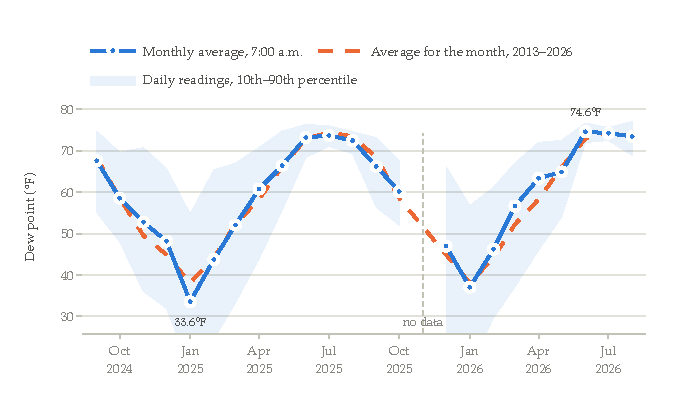
\includegraphics[width=\textwidth]{figures/dewpoint_history/dewpoint_history.pdf}
  \caption{Monthly average 7:00 a.m.\ dew point at Coulter Field, Bryan, Texas,
  September 2024 through August 2026. The shaded band is the 10th to 90th
  percentile of the individual daily 7:00 a.m.\ readings within each month, not
  an uncertainty interval about the mean. November 2025 is absent because the
  station reported on only five days that month.}
  \label{fig:history}
\end{figure}
\calcnote[inline]{FIG: \pth{figures/dewpoint\_history/}; reproduce with
\texttt{python figures/dewpoint\_history/make\_fig.py}, which writes
\pth{dewpoint\_history.pdf} from
\pth{analysis/dewpoint\_forecast/output/history\_window.csv} and
\pth{analysis/monthly\_dewpoint/output/climatology.csv}; shared style tokens
in \pth{figures/\_style.py}. The reference line is a plain average over the
2013--2026 record, not a WMO 30-year normal. Colors and mark specifications
follow the project's data-visualization conventions, recorded in
\pth{figures/\_style.py}: a validated blue and orange series pair here, a
single-hue blue ramp for the fan in Figure~\ref{fig:fan}.}

Twenty-three of the twenty-four months are observed. November 2025 is missing:
Coulter Field returned a valid 7:00 a.m.\ reading on only five days that month,
and those five days average 63.5\,\textdegree{}F against 52.6\,\textdegree{}F for
the full month at Easterwood, so the surviving days are badly unrepresentative
and the 20-day rule correctly excludes them.\calcnote{CALC: day counts and means
from \pth{output/daily\_dewpoint\_0700.csv}. DATA: the IEM download ends
2026-08-30 23:55 local, so the 31 August report was not yet archived at this
vintage.} August 2026 rests on 30 of 31 days, the record having been downloaded
before the month ended.

Two years is far too short a window to say anything about climate, and this
report does not try to. What the window does show is an unremarkable pair of
annual cycles. The mean over the twenty-three observed months is
59.4\,\textdegree{}F, which is 0.6\,\textdegree{}F above the station's own
2013--2026 average, and twelve of the twenty-three months sit above their
calendar-month average.\calcnote{CALC: \texttt{python}
\pth{analysis/dewpoint\_forecast/run.py}; block \texttt{[observed history]} of
\pth{output/model\_summary.txt}.} The extremes of the window are April 2026,
5.1\,\textdegree{}F above its calendar-month average, and January 2025,
4.5\,\textdegree{}F below. In levels, the window runs from 33.6\,\textdegree{}F
in January 2025 to 74.6\,\textdegree{}F in June 2026.

The feature of Figure~\ref{fig:history} that matters most for what follows is the
shaded band. Within-month dispersion of the daily readings is small in summer and
large in winter. In summer the morning air over central Texas is almost always
maritime tropical air off the Gulf, and its moisture content varies little from
day to day; in winter the same location alternates between that Gulf air and dry
continental air behind frontal passages, and the daily readings scatter
accordingly.\kbnote{KB: standard synoptic climatology of the western Gulf coastal
plain; check a regional climatology or synoptic text. High confidence in the
mechanism.} The same
asymmetry appears in the two-year record as a seasonal pattern in monthly mean
variability, and any honest forecast interval must reproduce it.

\section{A forecasting model for the monthly mean}
\label{sec:model}

\subsection{Specification}

Let $y_t$ be the monthly average 7:00 a.m.\ dew point in month $t$, let $m(t)$
be the calendar month, and let $\tau_t$ be time in years. The model is
%
\begin{align}
  y_t &= \mu_t + \sigma_t z_t, \label{eq:obs}\\
  \mu_t &= \beta_0 + \delta \tau_t
           + \sum_{k=1}^{K}\left[a_k \cos\frac{2\pi k\, m(t)}{12}
                               + b_k \sin\frac{2\pi k\, m(t)}{12}\right],
           \label{eq:mean}\\
  \log \sigma_t^2 &= \gamma_0
           + \sum_{l=1}^{L}\left[c_l \cos\frac{2\pi l\, m(t)}{12}
                               + d_l \sin\frac{2\pi l\, m(t)}{12}\right],
           \label{eq:scale}\\
  z_t &= \phi z_{t-1} + \varepsilon_t, \qquad
         \varepsilon_t \ \text{independent, mean zero}. \label{eq:ar}
\end{align}
%
Equation~\eqref{eq:mean} is a Fourier representation of the annual cycle in the
mean. Equation~\eqref{eq:scale} is the multiplicative heteroskedasticity model of
\citet{harvey1976multiplicative}, applied here to the calendar month rather than
to a regressor; it is what encodes the seasonal asymmetry in dispersion described
at the end of Section~\ref{sec:history}. Equation~\eqref{eq:ar} allows a
month-to-month carry-over in the standardized anomaly.

The numbers of harmonics $K$ and $L$ are chosen by the Bayesian information
criterion.\kbnote{ASSUME: BIC not AIC, wanting a parsimonious annual cycle rather
than a minimum in-sample fit. Section~\ref{sec:evaluation} shows that fixing
$K=2$ changes little out of sample.} Both select a
single harmonic. The mean equation is fit by ordinary least squares with
heteroskedasticity- and autocorrelation-consistent standard errors
\citep{newey1987simple}, using six lags.\kbnote{ASSUME: six HAC lags, conventional for monthly data. The
estimated $\phi$ below implies negligible autocorrelation past three months, so
this is not a sensitive choice.}

The scale equation's coefficients are estimated by regressing the log squared
residuals on the harmonic basis and removing the $-1.2704$ bias that
$\mathbb{E}[\log \chi^2_1] = \psi(1/2) + \log 2$ introduces.\kbnote{ASSUME: the $-1.2704$ correction is exact only under
normality. The fitted scale's level is afterwards renormalized to unit residual
variance, absorbing any resulting error in the constant.}

\subsection{Why the trend is not estimated from the Bryan record}

The trend $\delta$ requires a decision. Estimated freely on the Coulter Field
record, it comes out at $+1.61$\,\textdegree{}F per decade with a HAC standard
error of 0.71, apparently significant. It is not credible. Re-estimated as the
record lengthens, the coefficient falls monotonically from
$+7.25$\,\textdegree{}F per decade on data through August 2019 to
$+1.61$ through August 2026 (Table~\ref{tab:trend}). A genuine trend does not
behave that way; a low-frequency swing being read as a slope
does.\calcnote{CALC: \texttt{python} \pth{analysis/dewpoint\_forecast/run.py};
\pth{output/trend\_stability.csv}.}

\begin{table}[htbp]
  \centering
  \caption{The trend in the monthly mean 7:00 a.m.\ dew point, estimated on the
  Coulter Field record alone, as the sample lengthens.
  Degrees Fahrenheit per decade, HAC standard errors in parentheses.}
  \label{tab:trend}
  \begin{tabular}{lrr}
    \toprule
    Sample end & Months & Trend \\
    \midrule
    August 2019 &  75 & $+7.25$ \ (1.05) \\
    August 2020 &  87 & $+6.54$ \ (1.10) \\
    August 2021 &  99 & $+4.51$ \ (1.33) \\
    August 2022 & 111 & $+3.74$ \ (1.03) \\
    August 2023 & 123 & $+2.70$ \ (0.98) \\
    August 2024 & 135 & $+2.64$ \ (0.81) \\
    August 2025 & 147 & $+1.98$ \ (0.79) \\
    August 2026 & 158 & $+1.61$ \ (0.71) \\
    \bottomrule
  \end{tabular}
\end{table}

The same specification fit to the 368-month Easterwood record gives
$+0.559$\,\textdegree{}F per decade with a HAC standard error of
0.242.\calcnote{CALC: same command; block \texttt{[selected specification]} of
\pth{output/model\_summary.txt}.} That
figure is of the order reported for United States surface dew point in the
published literature, whereas the Coulter Field estimate is several times larger
\citep{brown2013trends, gaffen1999climatology}.\checknote{SRC: both papers are
cited for the order of magnitude of a U.S. dew point trend, not a Texas-specific
value. CHECK: I did not re-access either for a numerical coefficient, so the text
says only ``of the order reported''; read the trend tables of
\citet{brown2013trends} to compare numerically.}

The model therefore imposes $\delta$ at the Easterwood estimate rather than
estimating it on the Bryan record, carrying the standard error of that estimate
into the forecast simulation so the imposed trend is not treated as known. This
is legitimate because the two stations are 14.5 kilometers apart and their
monthly means correlate at 0.997: whatever the long-run slope at Easterwood is,
it is very nearly the slope at Coulter Field.
\kbnote[inline]{ASSUME: the Easterwood trend is treated as the Coulter Field
trend. The two records share a climate and an airmass regime, but they are
different instruments at different sites, so a genuine station-specific component
cannot be ruled out. The alternative of setting $\delta = 0$ was tested and
performs slightly worse out of sample (Section~\ref{sec:evaluation}), which is
why the trend is imposed rather than zeroed.}

The seasonal variance profile in equation~\eqref{eq:scale} is borrowed from
Easterwood on the same reasoning. Thirteen years supply only about thirteen
observations per calendar month, and $\log \chi^2_1$ has variance $\pi^2/2$, so
the shape of the seasonal variance profile is poorly determined at Coulter Field.
Only the shape is carried over; the level is renormalized to Coulter Field's own
residuals.\kbnote{ASSUME: the profile's shape is borrowed, its level is not.
Estimating the shape on the Bryan record is compared in
Section~\ref{sec:evaluation} and does slightly worse.}

\subsection{Estimates}

The fitted annual cycle in the mean runs from 41.7\,\textdegree{}F in January to
75.8\,\textdegree{}F in July, evaluated at the end of the sample. The fitted
standard deviation of the monthly mean runs from 1.57\,\textdegree{}F in July to
6.51\,\textdegree{}F in January, a ratio of just over four to
one.\calcnote{CALC: same command; \pth{output/seasonal\_profile.csv}.}
The autoregressive coefficient is
$\hat{\phi} = 0.217$ with a standard error of 0.078, so a month one standard
deviation above its seasonal mean is expected to be about a fifth of a standard
deviation above it the following month. A Ljung--Box test on the innovations at
twelve lags returns $p = 0.054$, which is weak evidence of remaining structure
rather than none.\calcnote{CALC: same command; block \texttt{[selected
specification]}.}
\checknote[inline]{CHECK: the Ljung--Box statistic is computed on residuals from a
fitted autoregression without the degrees-of-freedom adjustment for estimated
parameters, so its $p$-value is approximate. The statistic is borderline either
way, so this was not pursued; recompute with the adjustment if the distinction
matters.}

The predictive distribution is obtained by simulation rather than from a normal
formula. Each of 50{,}000 paths draws the mean-equation coefficients and $\phi$
from their estimated sampling distributions, draws the imposed trend from its
own, and resamples $\varepsilon$ from the empirical distribution of the fitted
innovations, in the spirit of the bootstrap autoregressive prediction intervals
of \citet{thombs1990bootstrap}. Resampling rather than drawing normal
shocks matters because the innovations are mildly right-skewed (0.23) and
leptokurtic (excess kurtosis 0.86).
\srcnote[inline]{SRC: \citet{thombs1990bootstrap} establish bootstrap prediction
intervals for autoregressions that account for parameter estimation error. The
procedure here follows that idea but is not their algorithm: parameters are drawn
from an asymptotic normal approximation rather than by resampling the estimation
itself. CALC: skewness and kurtosis from block \texttt{[selected specification]}
of \pth{analysis/dewpoint\_forecast/output/model\_summary.txt}; simulation
seed 20260831, and the code is deterministic given that seed.}

\section{The twelve-month forecast}
\label{sec:forecast}

Figure~\ref{fig:fan} presents the forecast as a fan chart, the presentational
convention introduced for the Bank of England's inflation projections
\citep{britton1998inflation} and since standard for density forecasts
\citep{wallis1999asymmetric, tay2000density}. Table~\ref{tab:forecast} gives the
same information numerically.

\begin{figure}[htbp]
  \centering
  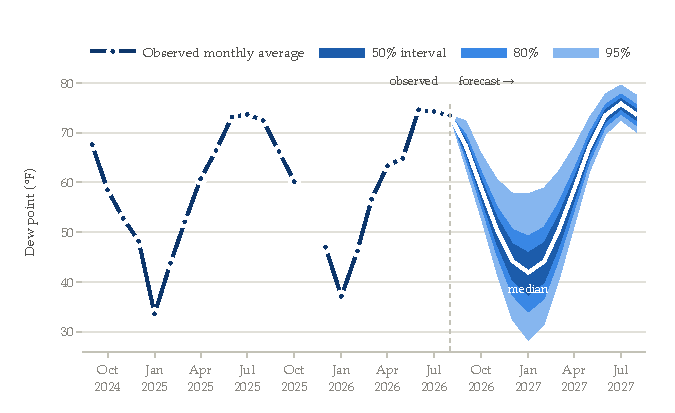
\includegraphics[width=\textwidth]{figures/dewpoint_fan/dewpoint_fan.pdf}
  \caption{Fan chart of the monthly average 7:00 a.m.\ dew point at Coulter
  Field, Bryan, Texas. Observed values through August 2026; simulated predictive
  distribution for September 2026 through August 2027. Bands are the central 50,
  80, and 95 percent of the predictive distribution, shaded darker where the
  outcome is more probable. The fan is anchored at the last observed month,
  whose value is known.}
  \label{fig:fan}
\end{figure}
\calcnote[inline]{FIG: \pth{figures/dewpoint\_fan/}; reproduce with
\texttt{python figures/dewpoint\_fan/make\_fig.py}, which writes
\pth{dewpoint\_fan.pdf} from
\pth{analysis/dewpoint\_forecast/output/forecast\_quantiles.csv} and
\pth{history\_window.csv}. Both figures share the y-axis range 26 to 82
\textdegree{}F so they can be read against each other.}

\begin{table}[htbp]
  \centering
  \caption{Predictive distribution of the monthly average 7:00 a.m.\ dew point at
  Coulter Field, Bryan, Texas, in degrees Fahrenheit. Central intervals from
  50{,}000 simulated paths.}
  \label{tab:forecast}
  \begin{tabular}{lrrrr}
    \toprule
    Month & Median & 50\% interval & 80\% interval & 95\% interval \\
    \midrule
    September 2026 & 67.3 & 65.9--68.6 & 64.8--69.7 & 63.1--72.4 \\
    October 2026   & 58.9 & 56.9--60.7 & 55.3--62.2 & 52.9--65.8 \\
    November 2026  & 50.4 & 47.5--53.0 & 45.3--55.1 & 41.7--60.6 \\
    December 2026  & 44.2 & 40.3--47.7 & 37.3--50.5 & 32.4--57.8 \\
    January 2027   & 41.9 & 37.4--45.9 & 34.0--49.2 & 28.3--57.7 \\
    February 2027  & 44.1 & 39.9--47.9 & 36.6--51.0 & 31.5--58.9 \\
    March 2027     & 50.2 & 46.9--53.3 & 44.3--55.8 & 40.0--62.1 \\
    April 2027     & 58.7 & 56.3--60.9 & 54.4--62.7 & 51.5--67.2 \\
    May 2027       & 67.2 & 65.6--68.8 & 64.2--70.1 & 62.2--73.1 \\
    June 2027      & 73.5 & 72.3--74.6 & 71.2--75.6 & 69.7--77.8 \\
    July 2027      & 75.8 & 74.7--76.8 & 73.8--77.7 & 72.5--79.5 \\
    August 2027    & 73.6 & 72.4--74.7 & 71.5--75.6 & 70.1--77.5 \\
    \bottomrule
  \end{tabular}
\end{table}
\calcnote[inline]{CALC: \pth{analysis/dewpoint\_forecast/}; reproduce with
\texttt{python analysis/dewpoint\_forecast/run.py}. Table values are the
\texttt{q025}, \texttt{q100}, \texttt{q250}, \texttt{q500}, \texttt{q750},
\texttt{q900}, and \texttt{q975} columns of
\pth{output/forecast\_quantiles.csv}, rounded to one decimal.}

The medians trace the seasonal cycle almost exactly, and this is the honest
result rather than a failure of effort. The standardized anomaly in the final
observed month, August 2026, is $-0.06$, essentially zero, so even the
first-month forecast has nothing to carry forward; and with
$\hat{\phi} = 0.217$, any carry-over would have decayed to under five percent of
its initial size within three months in any case.\calcnote{CALC: same command; $0.217^2 = 0.047$
and $0.217^3 = 0.010$. Final standardized residual in block \texttt{[selected
specification]}; interval widths in block \texttt{[forecast]}, line \texttt{80\%
interval width}.}

The information in Figure~\ref{fig:fan} is therefore almost entirely in the width
of the fan, which varies by a factor of four across the year. The 80~percent
interval spans 3.9\,\textdegree{}F for July 2027 and 15.2\,\textdegree{}F for
January 2027. A user planning
around next July's morning humidity can treat 75\,\textdegree{}F as close to a
sure thing; a user planning around next January's cannot usefully treat any value
between the middle thirties and the high forties as unlikely. The fan is also
visibly right-skewed in winter, its 95~percent upper bound sitting further from
the median than its lower bound, because the log-variance specification combined
with right-skewed innovations produces asymmetric intervals in the high-variance
months.

\section{Out-of-sample evaluation}
\label{sec:evaluation}

The model was evaluated by expanding-window pseudo-out-of-sample forecasting.
At each origin from August 2019 through July 2026, every quantity is
re-estimated from data dated on or before that origin, including the imposed
trend and the borrowed variance profile, and forecasts are issued for horizons
one through twelve months. That yields 930 forecast-target pairs. Specifications
are ranked by the continuous ranked probability score, which scores the whole
predictive distribution rather than a point forecast
\citep{hersbach2000decomposition, gneiting2007strictly}, and checked with the
coverage of the central intervals and the probability integral transform
\citep{diebold1998evaluating}.\calcnote{CALC:
\pth{analysis/dewpoint\_forecast/}. \pth{select\_spec.py} writes
\pth{spec\_comparison.txt}; \pth{run.py} writes
\pth{backtest\_by\_horizon.csv} and
\pth{backtest\_by\_month.csv}.}

Table~\ref{tab:specs} reports the comparison for the specifications that matter.
One difference dominates. Extrapolating the freely estimated trend raises CRPS by
0.38, or 21 percent, and leaves a mean forecast error of
$+1.67$\,\textdegree{}F: the model systematically forecasts too moist, exactly as
Table~\ref{tab:trend} predicts it would. Every specification that declines to
extrapolate that trend performs within noise of every other, across a band from
1.784 to 1.856.

\begin{table}[htbp]
  \centering
  \caption{Pseudo-out-of-sample comparison, 930 forecast-target pairs, origins
  August 2019 through July 2026. CRPS and errors in degrees Fahrenheit; nominal
  interval coverage is 0.50, 0.80, and 0.95. The selected specification is the
  first row.}
  \label{tab:specs}
  \begin{tabular}{llrrrrr}
    \toprule
    Trend & Variance profile & CRPS & MAE & Bias & Cov.\ 80\% & Cov.\ 95\% \\
    \midrule
    Anchored & Easterwood & 1.784 & 2.504 & $-0.26$ & 0.898 & 0.970 \\
    None     & Easterwood & 1.796 & 2.520 & $-0.44$ & 0.900 & 0.975 \\
    Anchored & Coulter    & 1.833 & 2.567 & $-0.14$ & 0.902 & 0.973 \\
    None     & Coulter    & 1.844 & 2.591 & $-0.34$ & 0.899 & 0.971 \\
    Free     & Coulter    & 2.167 & 3.008 & $+1.67$ & 0.697 & 0.926 \\
    \bottomrule
  \end{tabular}
\end{table}
\calcnote[inline]{CALC: rows selected from
\pth{analysis/dewpoint\_forecast/output/spec\_comparison.csv}, which contains
fourteen specifications; the five shown isolate the two decisions discussed in
Section~\ref{sec:model}. The omitted rows vary the number of harmonics and the
weighting of the mean regression and span CRPS 1.789 to 1.856. The 21 percent
figure quoted in the text is $(2.1665 - 1.7844)/1.7844$.}

Three further results deserve statement.

First, the autoregressive term earns nothing. Pooled across horizons the model
scores 1.783 with it and 1.775 without; at a one-month horizon it scores 1.887
with and 1.843 without.\calcnote{CALC: block \texttt{[backtest]} of
\pth{output/model\_summary.txt}, columns \texttt{CRPS} and \texttt{CRPS(no
AR)}.} The in-sample $\hat\phi = 0.217$ is real but too small to survive
estimation error out of sample. The term is retained because it is the
pre-specified structure and because removing it on the strength of a difference
this small, measured on heavily overlapping pairs, would itself be a form of
overfitting; but no claim is made that it improves the forecast.

Second, the intervals are somewhat too wide rather than too narrow. Pooled
coverage of the 50, 80, and 95 percent intervals is 0.568, 0.896, and 0.968
against nominal 0.50, 0.80, and 0.95. Restricting to origins from August 2023
onward, where the training sample is closer in length to the one actually used,
coverage is 0.497, 0.867, and 1.000 on 354 pairs.\calcnote{CALC: block
\texttt{[backtest]} of \pth{output/model\_summary.txt}, pooled line and the
\texttt{origins 2023-08 onward} line.} Erring wide is the conservative direction
for a fan chart, but readers should understand that the bands in
Figure~\ref{fig:fan} are, if anything, a little generous.

Third, accuracy does not degrade with horizon at all. Mean absolute error is
2.70\,\textdegree{}F at one month and 2.44\,\textdegree{}F at twelve, and does
not trend in between.\calcnote{CALC:
\pth{output/backtest\_by\_horizon.csv}.} That is the same finding as the first,
seen from another angle: nothing in this month's observation tells you much about
next month's, so a twelve-month-ahead forecast is no harder than a one-month
one.

\section{Limitations}
\label{sec:limitations}

The seasonal mean uses a single harmonic, which BIC selects and which the
out-of-sample comparison does not reject, but which cannot reproduce the sharper
minimum the data show in January. In the backtest the model runs
$+2.99$\,\textdegree{}F too moist in January and $-3.05$ and
$-2.86$\,\textdegree{}F too dry in March and December, against a mean error
below 1.2\,\textdegree{}F in absolute value in every month from April through
November.\calcnote{CALC: \pth{output/backtest\_by\_month.csv}.} Adding a second harmonic reduces those
winter biases but does not improve the overall score, because the winter months
where it helps are also the months with the widest intervals, where a mean shift
of two or three degrees costs little. Users interested specifically in
midwinter should treat the December through March medians in
Table~\ref{tab:forecast} as carrying a systematic error of a few degrees whose
sign is known.

The forecast conditions on no information beyond the station's own history. It
uses no sea surface temperature state, no El Niño--Southern Oscillation index,
and no numerical weather prediction or seasonal model output, any of which would
plausibly narrow the winter intervals where the uncertainty actually
lies.
\kbnote[inline]{KB: ENSO state is a recognized predictor of Gulf-coast winter
moisture and precipitation; a reviewer should check a seasonal forecasting
reference for the strength of the relationship at this location. Moderate
confidence: the relationship is well established, its magnitude at Bryan
specifically is not something I verified. CHECK: no attempt was made to quantify
how much an ENSO predictor would improve these forecasts, so ``would plausibly
narrow'' is a judgment, not a result.}

The record is short and single-sited. Thirteen years at Coulter Field cannot
distinguish a trend from a low-frequency swing, which is precisely the problem
Section~\ref{sec:model} works around rather than solves. Nor has any check been
made for instrumentation changes, site changes, or calibration drift at either
station, any of which would show up as an apparent
trend.
\checknote[inline]{CHECK: I did not consult station history metadata for KCFD or
KCLL. NOAA maintains such records \citep{noaa1998asos}, and they should be
checked before any trend claim in this report is relied upon. This is the
likeliest source of a material error in the imposed trend.}

Finally, the specification was selected using the same backtest that then reports
its performance. The 930 pairs overlap heavily, so the apparent precision of the
comparison in Table~\ref{tab:specs} is overstated, and the reported scores for
the selected model are optimistic by an unquantified
amount.\kbnote{ASSUME: the standard selection-bias caveat. Mitigated, not
removed, by the decisive comparison being a 20 percent CRPS gap with a mechanism
visible in Table~\ref{tab:trend}, not a marginal score difference.}

\printbibliography

% Index of all provenance notes, last in the document. A no-op in the clean
% build, optional argument and all.
\listoftodos[Review notes]

\end{document}
